\sectionSlide{Language popularity}{languages-popularity}{\paperwidth}{t}

\slide{C++ users}{
    \begin{columns}
        \begin{column}{0.5\textwidth}
            {\small 
                \begin{table}
                    %\caption{C++ users}
                    \begin{tabular}{|l|r|}
                        \hline \textbf{Date} & \textbf{Estimated users} \\
                        \hline 
                        \hline 1979 & 1 \\
                        \hline 1980 & 16 \\
                        \hline 1981 & 38 \\
                        \hline 1982 & 85 \\
                        \hline 1983 & ??+2 \\
                        \hline 1984 & ??+50 \\
                        \hline 1985 & 500 \\
                        \hline 1986 & 2 000 \\
                        \hline 1987 & 4 000 \\
                        \hline 1988 & 15 000 \\
                        \hline 1989 & 50 000 \\
                        \hline 1990 & 150 000 \\
                        \hline 1991 & 400 000 \\
                        \hline
                    \end{tabular}
            \end{table}}        
        \end{column}
        \begin{column}{0.5\textwidth}
            \pause
            Main users:
            \begin{itemize}[<+->]
                \item Bjarne,
                \item Bjarne's colleagues from AT\&T Bell Labs,
                \item universities,
                \item HP, IBM, AT\&T, DEC,
                \item Borland,
                \item Later: Microsoft, Apple,
                \item Now: Google, Facebook
            \end{itemize}
        \end{column}
    \end{columns}
}


\slide{C++ users}{
    \centering 
    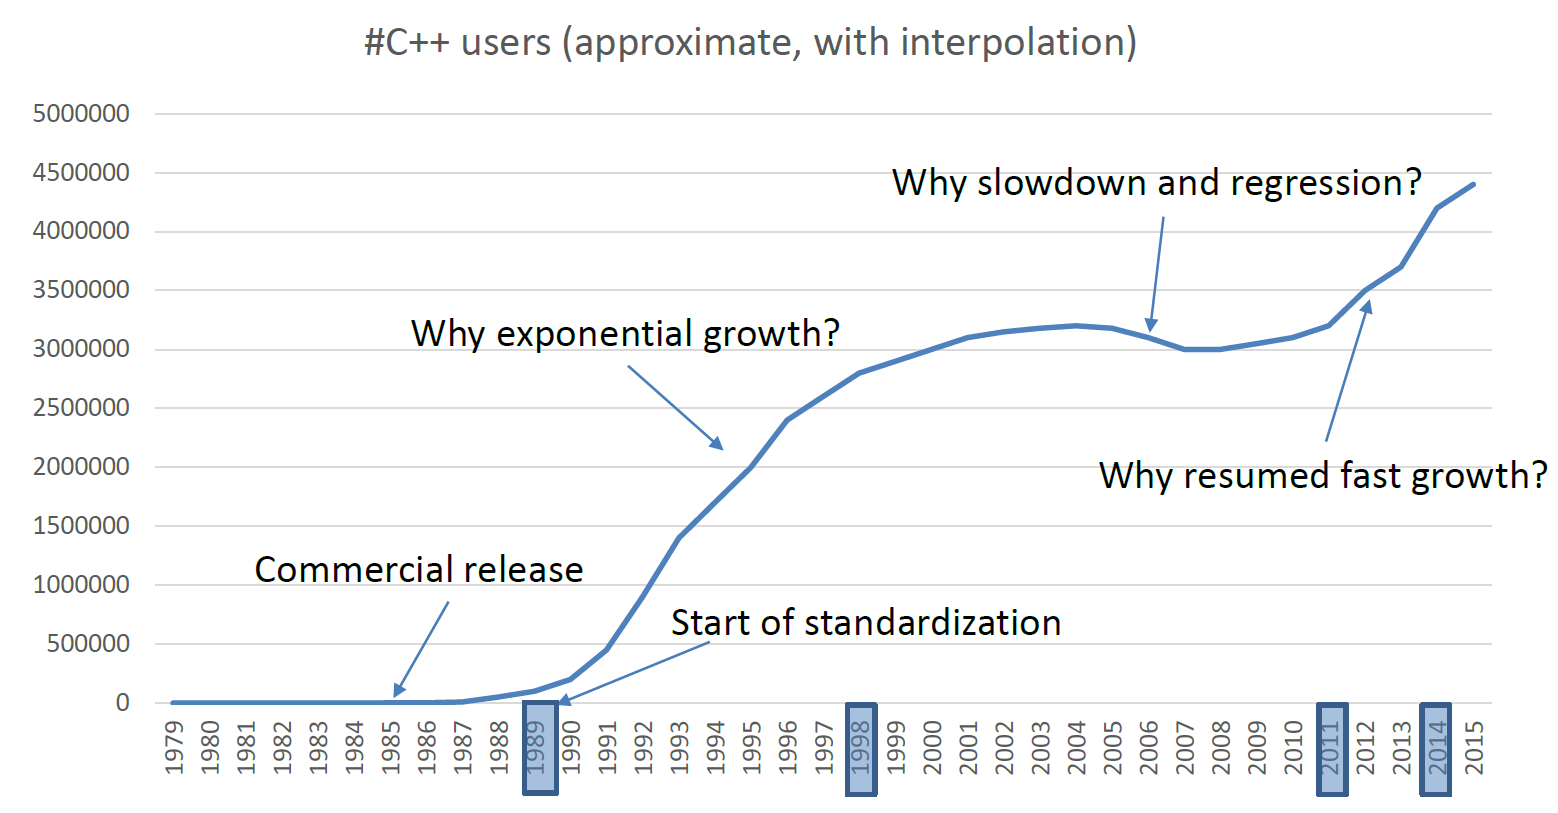
\includegraphics[height=0.8\paperheight]{cpp_users}
}


\slide{TIOBE}{
    \only<1>{
        \begin{block}{TIOBE index}
            \textbf{The TIOBE Programming Community} index is an indicator of the popularity of programming languages. The index is updated once a month. Popular search engines such as \textbf{Google, Bing, Yahoo!, Wikipedia, Amazon, YouTube} and \textbf{Baidu} are used to calculate the ratings. Search phrase is \textbf{"language programming"} \\
            Webpage: \url{http://www.tiobe.com/tiobe-index//}
        \end{block}
    }
    \centering 
    \includegraphics<2>[height=0.7\paperheight]{tiobe-array}
    \includegraphics<3>[height=0.7\paperheight]{tiobe-graph}
}


\slide{PYPL}{
    \only<1>{
        \begin{block}{PYPL index}
            \textbf{The PYPL PopularitY of Programming Language} Index is created by analyzing how often \textbf{language tutorials} are searched on Google: the more a language tutorial is searched, the more popular the language is assumed to be. It is a leading indicator. The raw data comes from \textbf{Google Trends}. \\
            Webpage: \url{http://pypl.github.io/PYPL.html}  
        \end{block}
    }
    \centering 
    \includegraphics<2>[height=0.8\paperheight]{pypl-array}
    \includegraphics<3>[height=0.8\paperheight]{pypl-graph}
}


\slide{codeeval}{
    \only<1>{
        \begin{block}{codeeval MPCL}
            \textbf{"Most Popular Coding Languages"} is based on hundreds of thousands of data points we've collected by processing over 1,200,000+ \textbf{challenge submissions on codeeval.com} in (now) 26 different programming languages. \\
            Webpage: \url{http://blog.codeeval.com/}  
        \end{block}
    }
    \centering 
    \includegraphics<2>[height=0.83\paperheight]{codeeval2016}
    \includegraphics<3>[height=0.83\paperheight]{codeeval2015}
%    \includegraphics<4>[height=0.34\paperheight]{codeeval2014}
}


\slide{langpop.corger.nl}{
    \begin{block}{Programming Language Popularity Chart}
        The data from \textbf{GitHub} that is displayed in the chart is based on results from actively polling the GitHub events API. \\
        Results from \textbf{Stack Overflow} are based on the number of times that a tag for a certain language is applied, together with the applied count of the synonyms of that language. This data is refreshed every four hours in order to keep it up-to-date. \\
        Webpage: \url{http://langpop.corger.nl/}  
    \end{block}
}
\imageSlide{langpop-graph}


\slide{C++ is not dead!}{
    \begin{columns}
        \begin{column}{0.6\textwidth}
            \begin{itemize}
                \item In the worst case C++ is on 7th place
                \item In the best case C++ is on 3rd place
                \item C++ is one of the most popular languages!
            \end{itemize}
        \end{column}
        \begin{column}{0.4\textwidth}
            
\includegraphics[height=0.8\paperheight]{bjarne-stroustrup}
        \end{column}
    \end{columns}
}